\documentclass[sigconf]{acmart}
\settopmatter{printacmref=false, printccs=false, printfolios=true}
\renewcommand\footnotetextcopyrightpermission[1]{}


\usepackage{booktabs} % For formal tables

\usepackage{wrapfig}

\begin{document}
\title{Concurrency and Parallelism 2023-24 \break Iterative Histogram Equalization}


\author{Cláudio Guerra}
\email{c.guerra@campus.fct.unl.pt}

\author{Tomás Mondim}
\email{t.mondim@campus.fct.unl.pt}


\begin{abstract}
This paper explores the implementation and performance analysis of iterative histogram equalization using different parallel computing techniques, including OpenMP and CUDA, to optimize image processing tasks. Through experimentation and comparison with sequential processing, we aim to identify the most efficient approach for large-scale image manipulation.
\end{abstract}

% We no longer use \terms command
%\terms{Theory}

\keywords{CUDA, NVIDIA, OpenMP, Multi-Processing, Graphics, Histogram Equalization}


\maketitle

\section{Introduction}

Histogram equalization is a technique used in image processing to enhance the contrast of an image. This method works by effectively spreading out the most frequent intensity values, resulting in an image with enhanced contrast. The goal is to obtain an output image with a uniform histogram, meaning all intensity values should ideally have an equal number of pixels. This transformation helps in highlighting the features of an image, making it more visually appealing and easier to analyze.

Iterative histogram equalization is an extension of this concept, where the process of histogram equalization is performed multiple times. By repeatedly applying histogram equalization, we can further refine the contrast enhancement of the image. This iterative approach can help in achieving better results, especially for images with complex histograms.

OpenMP (Open Multi-Processing) is an API that supports multi-platform shared memory multiprocessing programming in C, C++, and Fortran. It allows developers to write parallel code by using compiler directives, library routines, and environment variables. OpenMP is designed to simplify the development of parallel applications by providing a straightforward way to parallelize loops and sections of code.

CUDA is a powerful programming model and parallel computing platform crafted by NVIDIA. This platform aims to accelerate applications by harnessing the immense parallel architecture of NVIDIA GPUs.

Our project was divided into two main stages, each leveraging different parallel computing technologies: OpenMP and CUDA. The primary objective was to accelerate the process of iterative histogram equalization using these technologies, thereby significantly reducing the time required for processing large images.

\subsection{Hardware}

For the development of this project, the final code was run on a computer with 16 GB of RAM at 3200mHz, an AMD 7 5700X CPU and an NVIDIA RTX 4070 Super on Pop\_OS! 22.04 and CUDA Toolkit 12.5.

\section{Stage 1}

To improve readability, maintainability, and the parallelization of the code, we divided the histogram equalization functionality into several modular functions. This modular approach not only makes it easier to understand the flow of data and operations but also allows us to identify and focus on specific functions that may be problematic in terms of performance or correctness.

We then focused our parallelization efforts on the functions greyscale\_image, create\_histogram, and color\_correct\_and\_output, which present performance challenges due to their sequential nature and high computational complexity.

\begin{center}
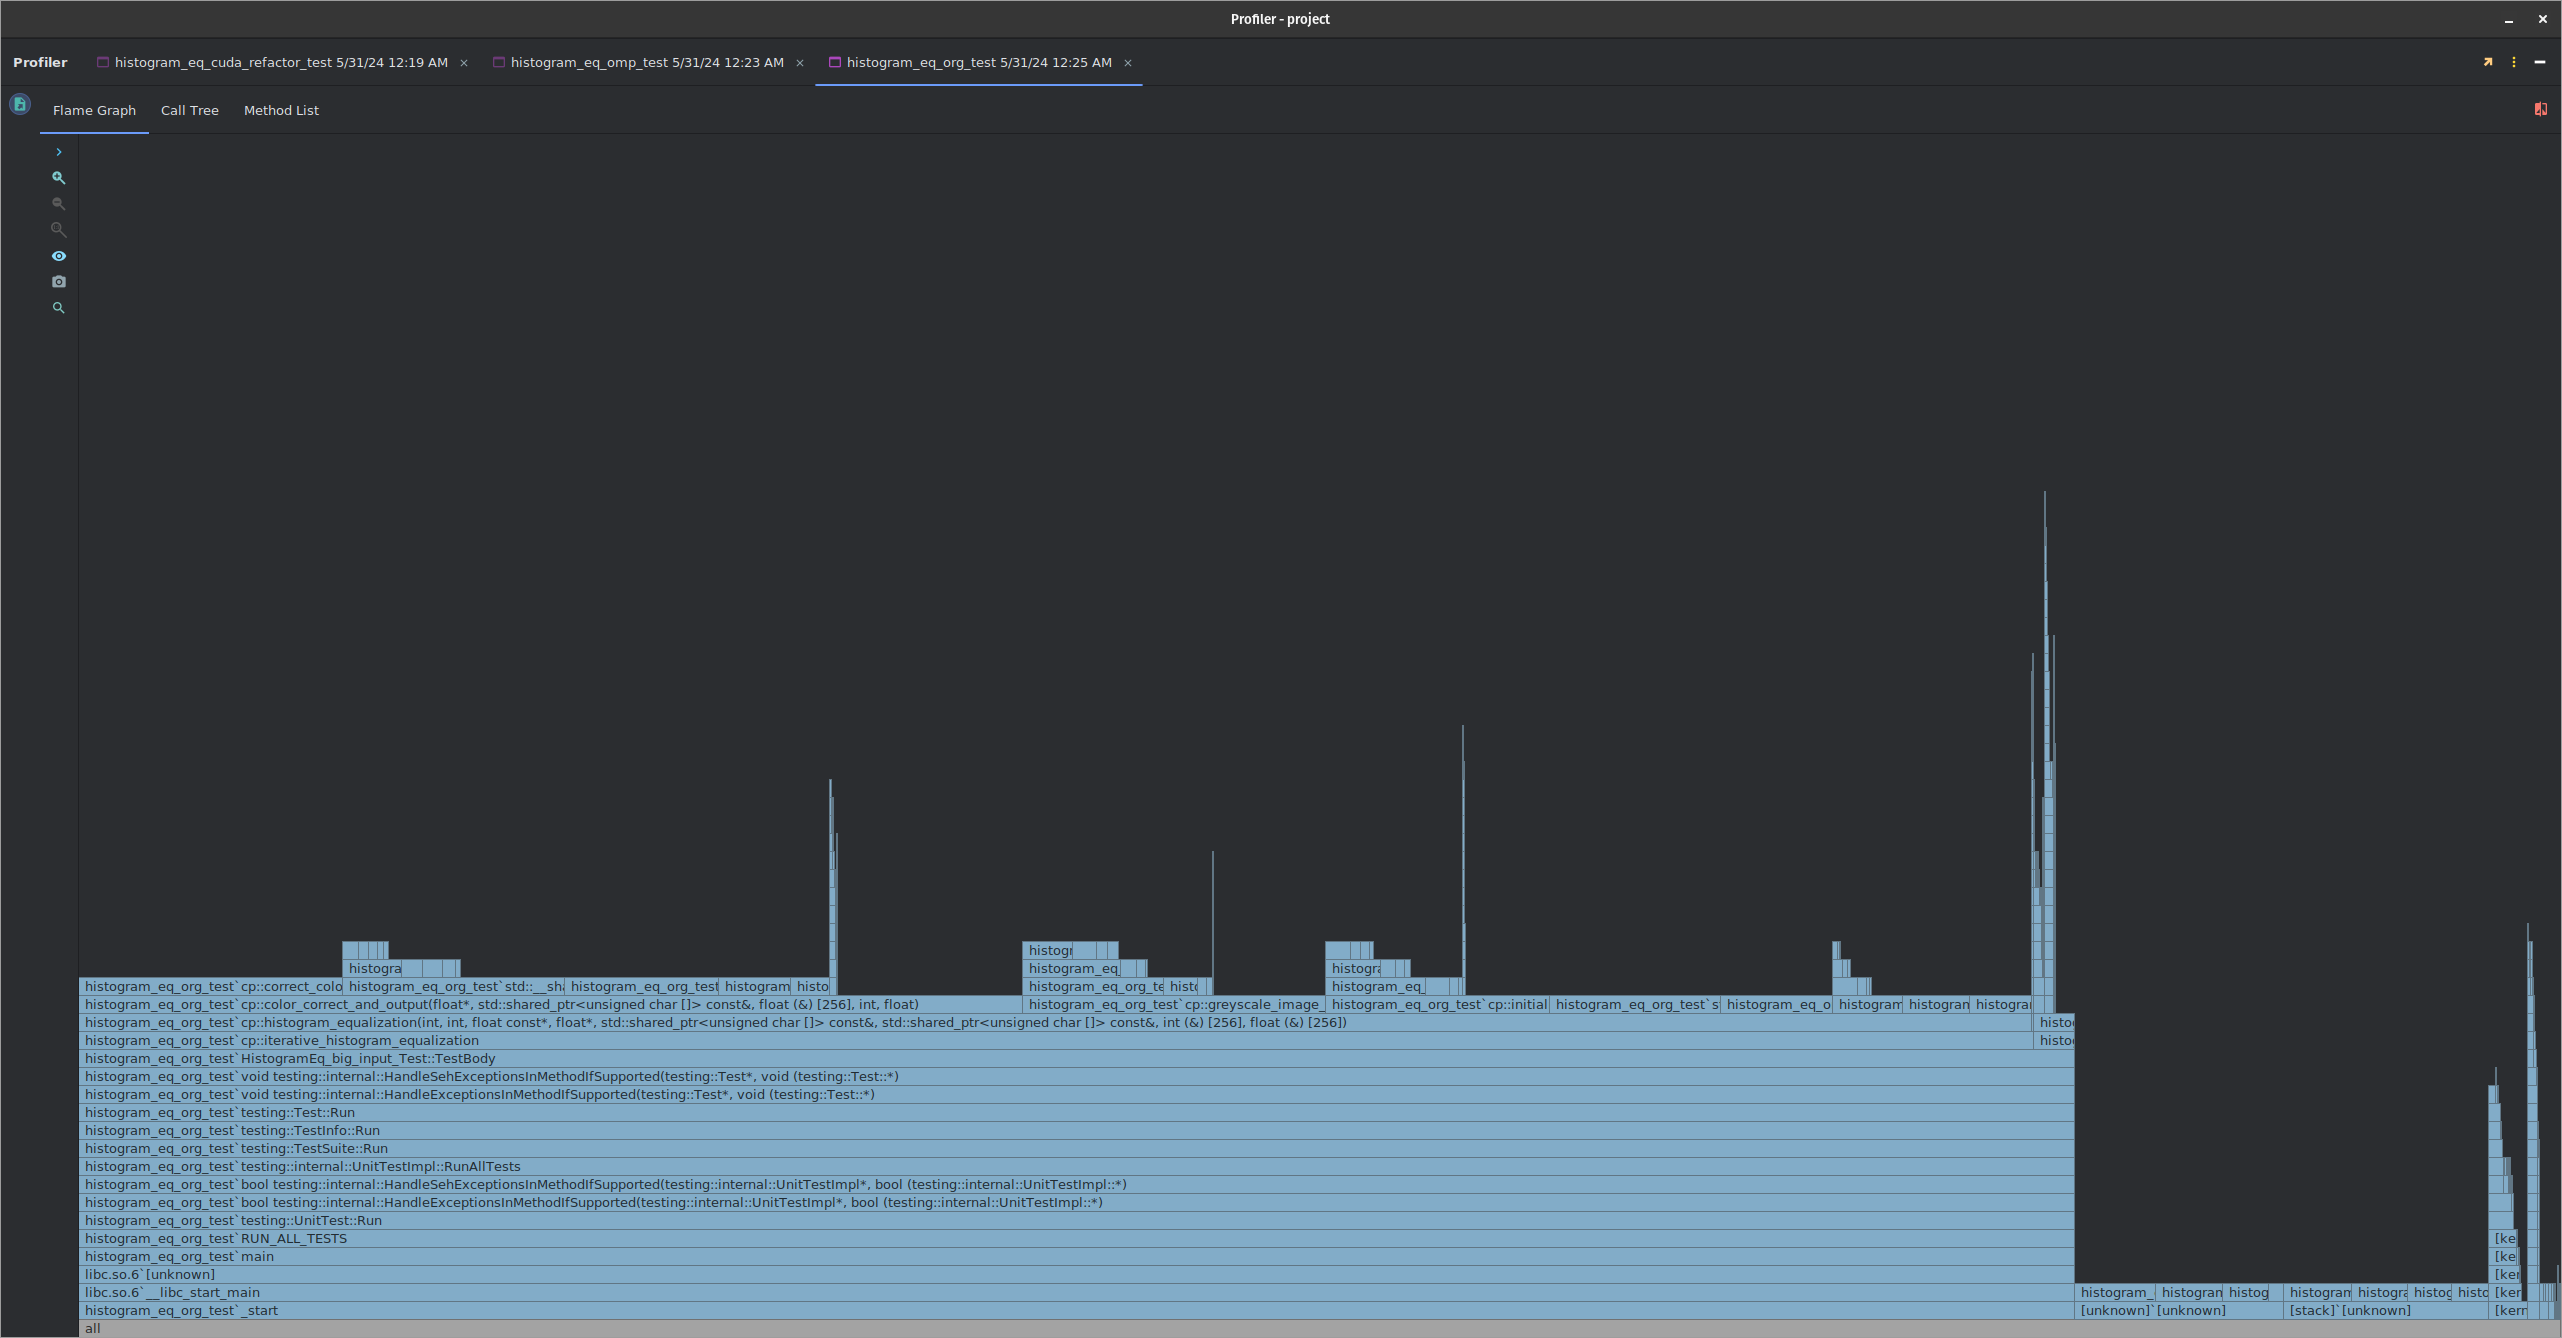
\includegraphics[width=0.8\linewidth]{vizs/original_function_profiler.png}
\captionof{figure}{CLion Profiler for the sequential version of the code.}
\label{sequential_profiler}
\end{center}

During this stage, we utilized OpenMP to parallelize various functions and loops.

Originally, the initialization of the uchar\_image array was done sequentially in a for loop. We modified it by adding a \#pragma omp parallel for to parallelize the loop, allowing multiple processor cores to initialize the array simultaneously.


The conversion of a color image to grayscale and the creation of the histogram were originally performed using nested for loops. We combined these operations into a single loop and used \#pragma omp parallel for reduction(+ : histogram) to parallelize the conversion and histogram creation, efficiently summing the histogram values and speeding up the processing by distributing the work across multiple cores.

\begin{center}
\centering
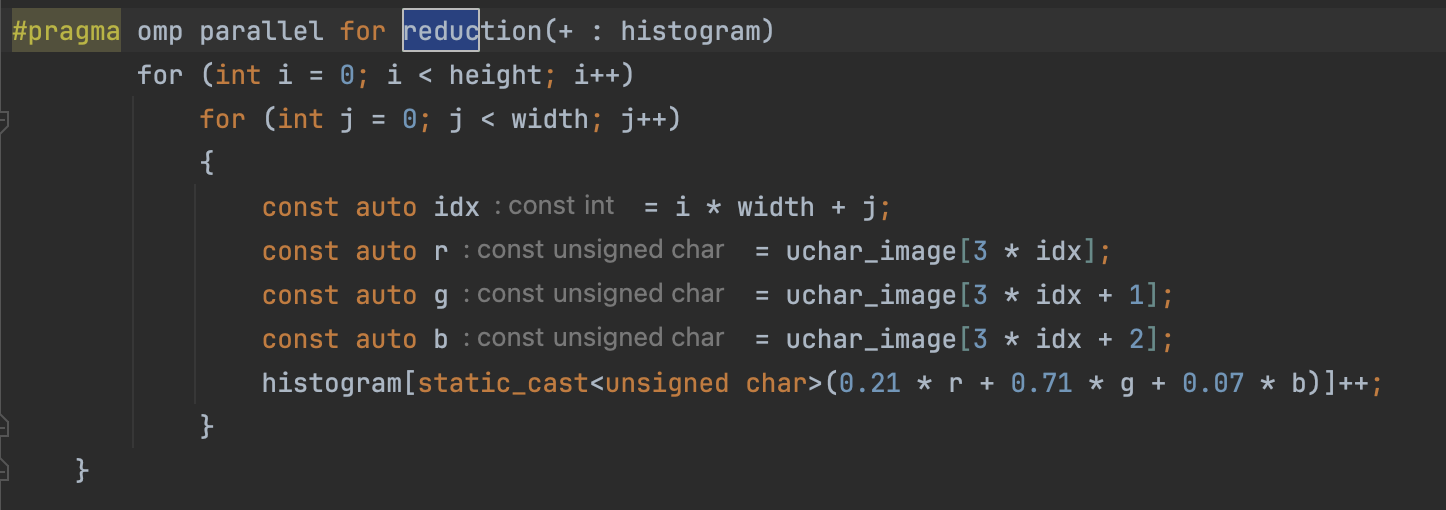
\includegraphics[width=0.8\linewidth]{vizs/histogram_openmp.png}
\captionof{figure}{The modified loop that joined the histogram and the grayscale functions together.}
\label{histogram_loop}
\end{center}

The color correction and output image production were performed sequentially in two for loops. We added \#pragma omp parallel for to parallelize both loops, speeding up the conversion of corrected values to the output image.
\section{Stage 2}
At this stage, we used CUDA to parallelize the main processes of the histogram equalization algorithm, substantially improving the efficiency of image processing.

In CUDA, threads are organized in blocks and execute identical instructions, although each thread can manipulate distinct data points. Warps represent groups of threads functioning synchronously, executing the same instruction simultaneously. These warps, acting as hardware execution units in GPUs, maintain lockstep execution but can switch to different warps when encountering memory operations or divergent control flow.

This understanding is crucial because when executing a kernel in CUDA, specifying the number of blocks and threads per block directly impacts the parallelism and resource utilization of the GPU, ultimately affecting performance and efficiency. For optimal performance, threadsPerBlock is set at 256, following NVIDIA's recommendations. This ensures efficient use of each streaming multiprocessor on the GPU. The calculation for blocksPerGrid ensures that there are enough blocks to cover all data elements, maximizing GPU utilization and ensuring no data is left unprocessed.

We implemented functions to allocate and free memory on the GPU, ensuring the necessary data is available for the CUDA kernels. A CUDA kernel was created to initialize the uchar\_image array and another to convert the color image to grayscale on the GPU. The CUB library was used to efficiently create the histogram on the GPU.

Additionally, a CUDA kernel was developed to apply color correction and generate the output image. These CUDA functions were then integrated into a histogram equalization workflow within static void histogram\_equalization. Finally, iterative histogram equalization was implemented using these CUDA functions in bImage\_t iterative\_histogram\_equalization.

\section{Performance Analysis}

In the realm of performance analysis, our focus centered on examining three distinct types of code: the sequential version, which can be run with vectorization either enabled or disabled; CUDA, a programming language facilitating General-Purpose computing on Graphics Processing Units (GPUs); and OpenMP, a library designed to facilitate parallel processing on shared-memory architectures. 

\subsection{Sequential}

To examine the sequential code's performance with and without optimization flags, we included the following segment in our CMakeLists.txt file, showcased in Fig. \ref{vectorization_toggle}.

\begin{center}
    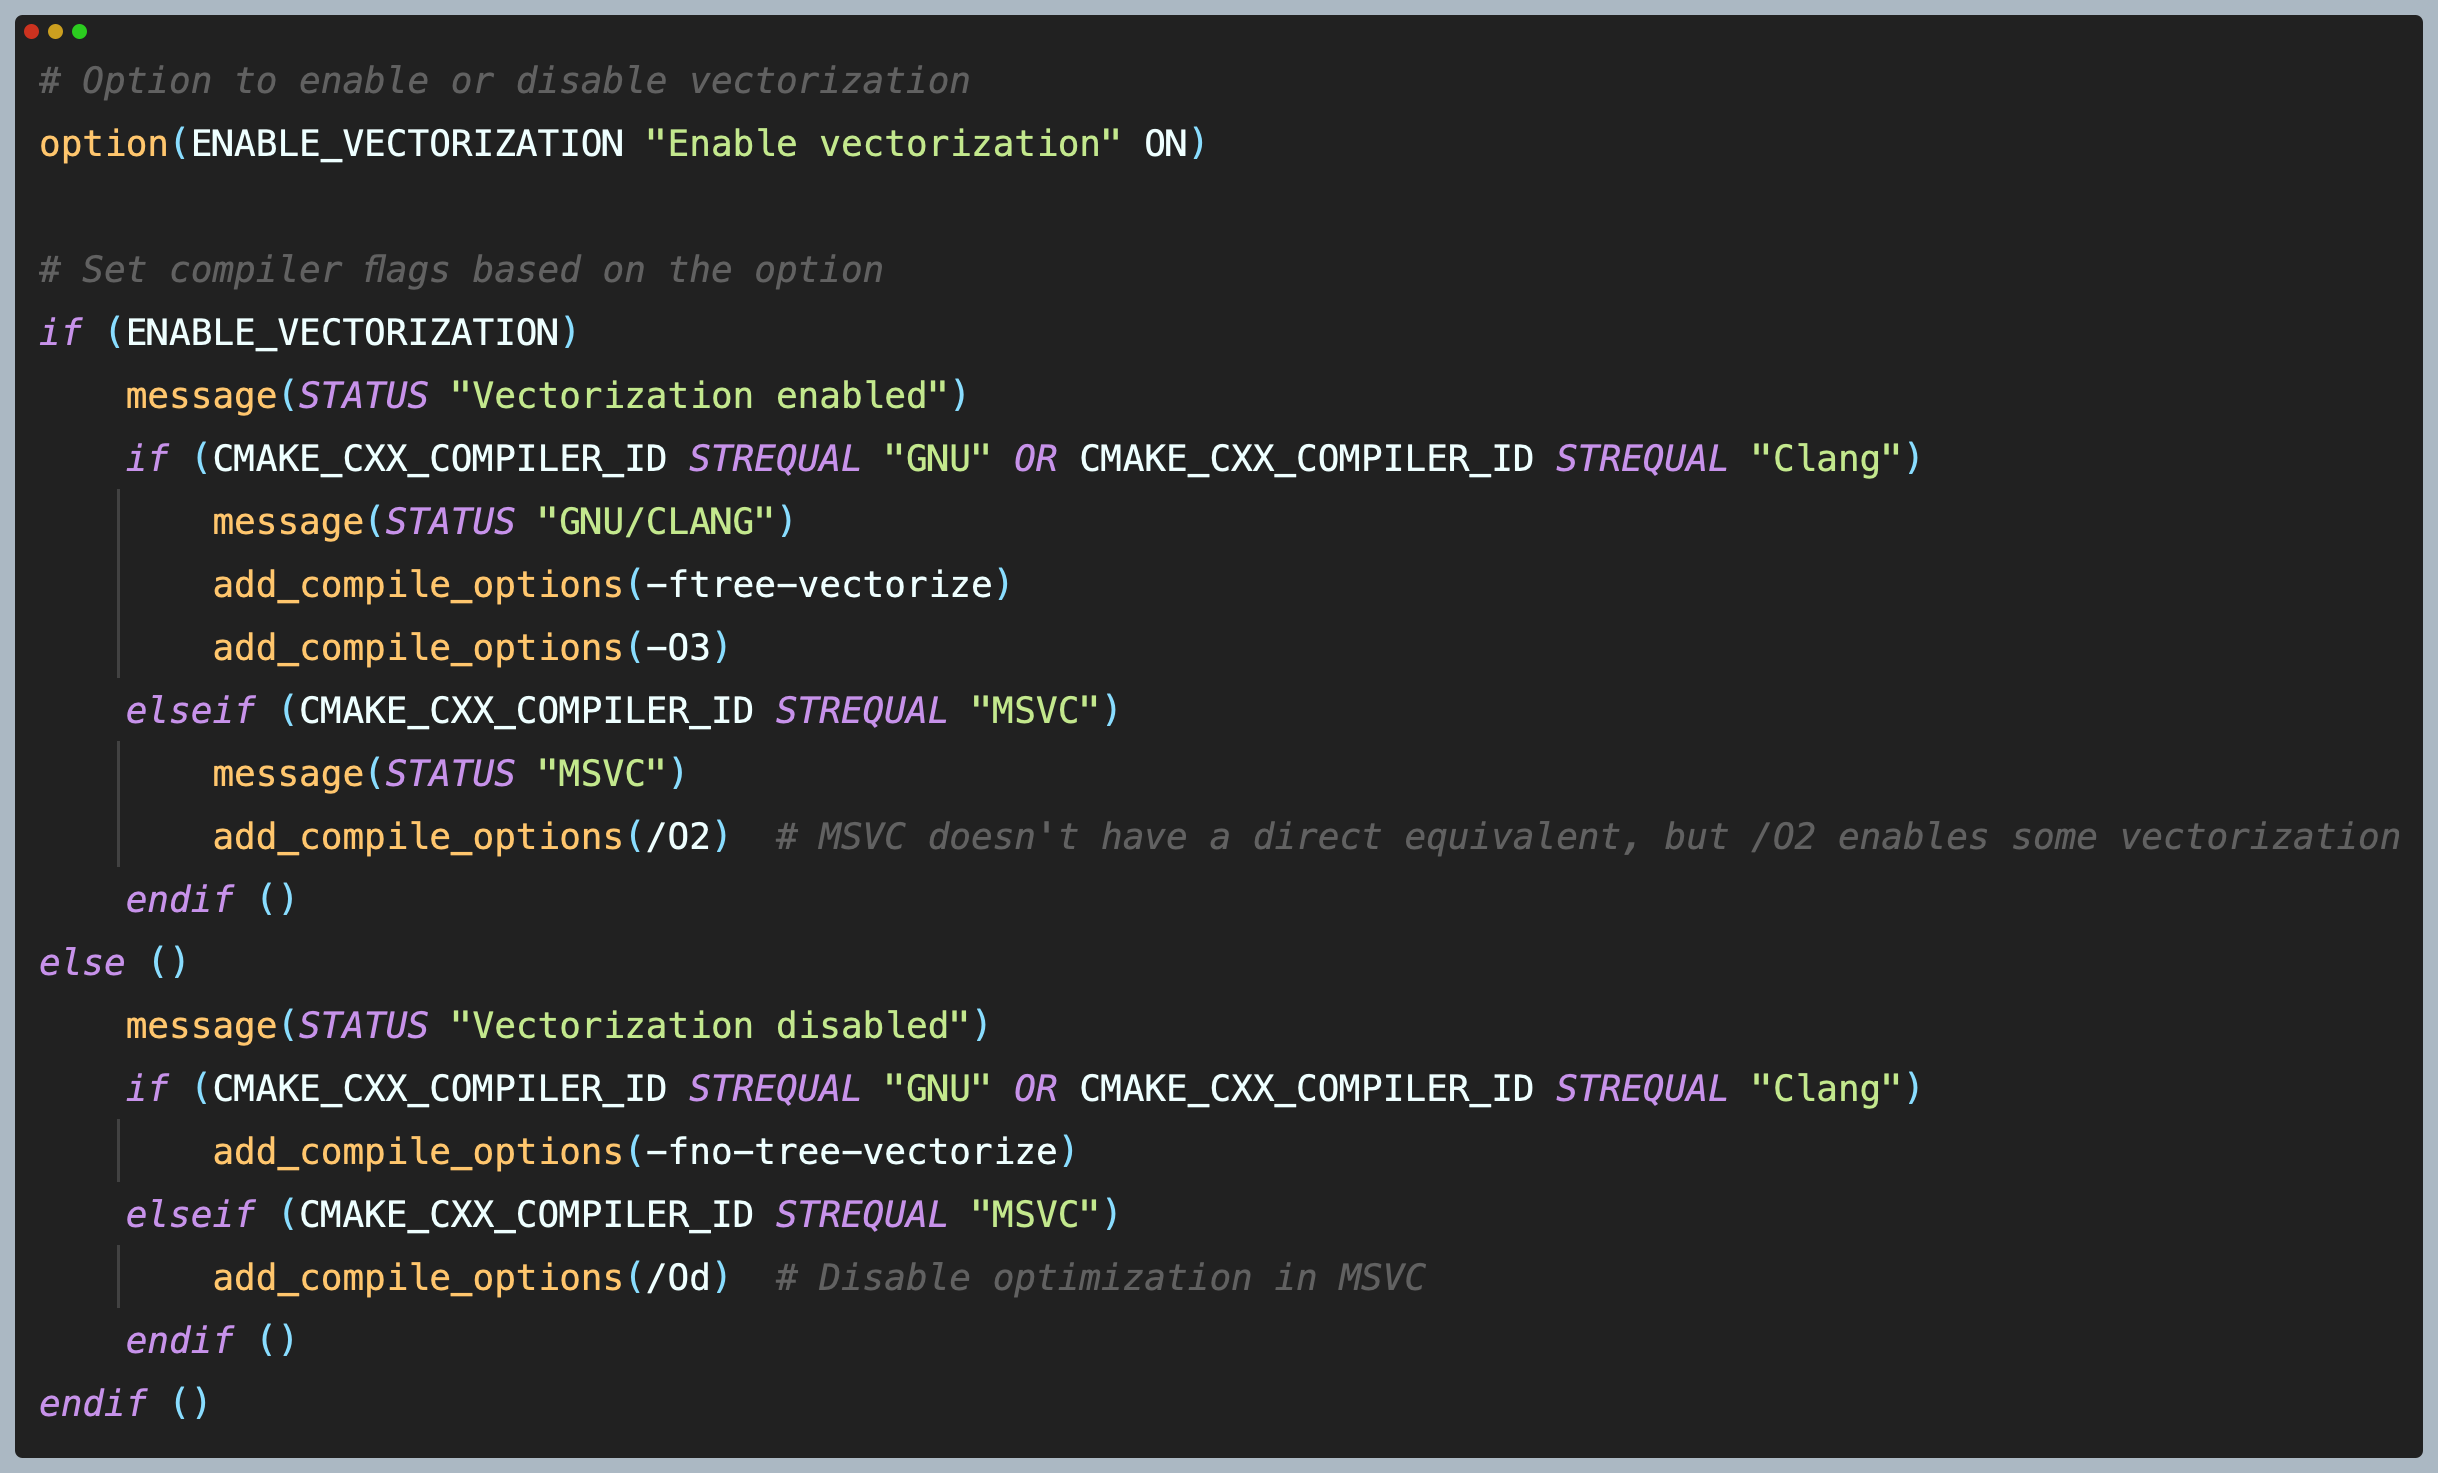
\includegraphics[width=0.8\linewidth]{vizs/vectorization_code.png}
    \captionof{figure}{Showcasing how vectorization was toggled on and off.}
    \label{vectorization_toggle}
\end{center}

This code snippet allows toggling vectorization optimizations on or off and adjusts compiler flags accordingly for GNU, Clang, and MSVC compilers. However, we only tested it with GNU.


Once we had the toggling set up, we ran both sequential and non-sequential versions. Initially, for images with resolutions below 1024x1024 (inclusive), the disparity between the results of optimized and non-optimized versions wasn't significant. But predictably, without any compiler optimizations, the non-optimized version of the code was painfully slow. There were instances where the optimized version could process an image in 0.5 seconds, while the non-optimized one took 6 seconds – a whopping 12 times slower, as showcased in Fig \ref{processing_time_vector_and_no_vector}.

\begin{center}
    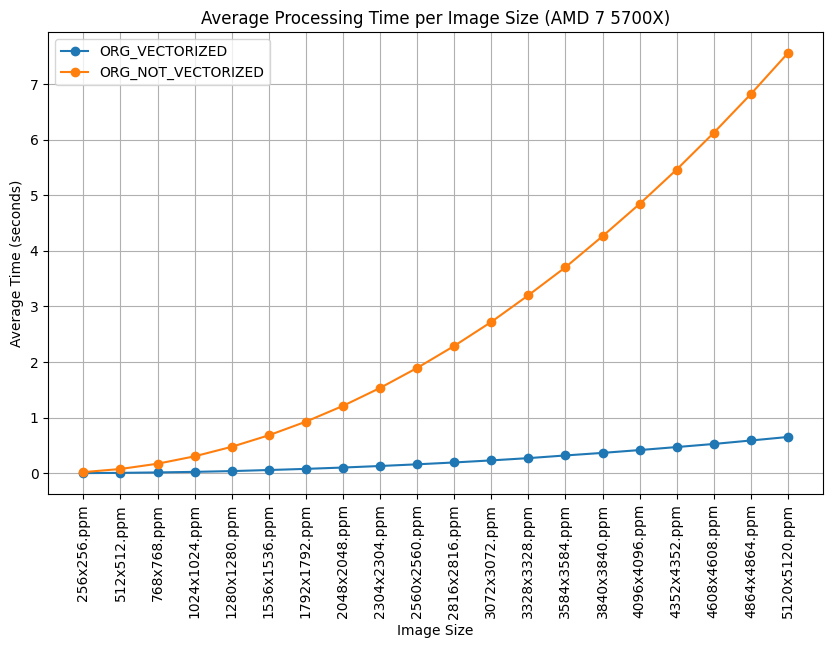
\includegraphics[width=0.8\linewidth]{vizs/amd_output_org.png}
    \captionof{figure}{Average time spent in 4 iterations for various image sizes. Optimized and non-optimized version of sequential version only. AMD 7 5700X.}
    \label{processing_time_vector_and_no_vector}
\end{center}


This observation already underscores the advantages optimization flags can bring to code, as evidenced by the significant performance improvements observed by just setting up two flags.

For the sake of simplicity, we won't discuss the non-optimized version further, and we kept the optimization flag ON for the other implementations.


\subsection{OpenMP}

For OpenMP, as we can see in Fig. \ref{openmp_and_org}, we get an interesting result. 

\begin{center}
    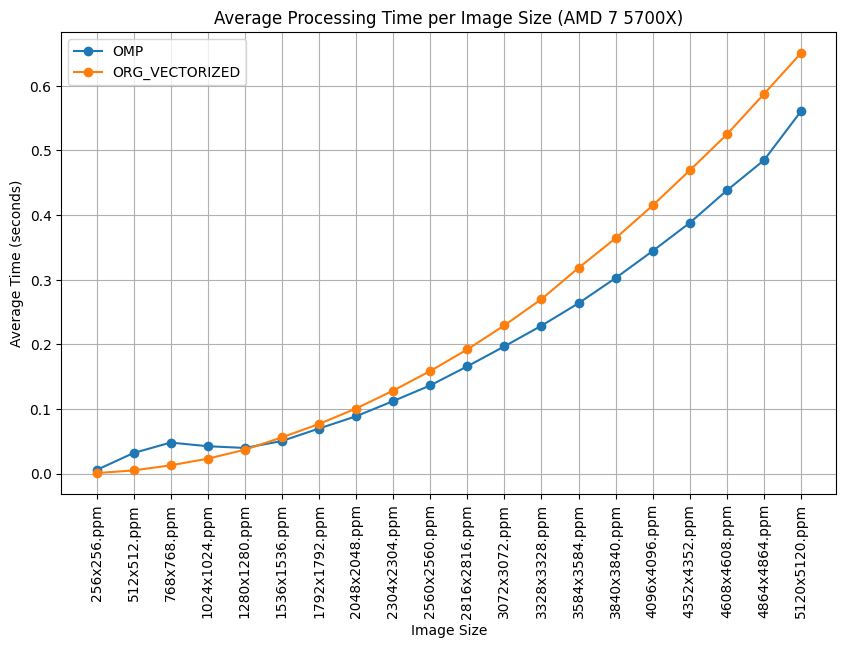
\includegraphics[width=0.8\linewidth]{vizs/omp_and_org.png}
    \captionof{figure}{Average time spent in 4 iterations for various image sizes. Optimized sequential version and OpenMP only. AMD 7 5700X.}
    \label{openmp_and_org}
\end{center}

Initially, we anticipated consistent performance gains across all image sizes due to OpenMP's focus on parallelizing code and utilizing multicore processors. However, after analyzing the data, we noticed that the optimized sequential code outperforms the OpenMP version in the initial image sizes, particularly those below 1536x1536. From these resolution upwards, however, the OpenMP library begins to pay dividends, consistently staying below the original sequential version, even with all optimizations enabled. 

We have two guesses as to this.

\begin{itemize}
    \item The overhead of managing threads outweighs the cost of actually processing the image for those first few small resolutions.
    \item When examining Fig. \ref{omp_profiler}, we observe a significant bar in our \textit{correct\_color\_and\_output} function. This suggests that the function may not be fully optimized and could benefit from enhancements such as a reduction or other optimizations that may have been overlooked. Nonetheless, the OpenMP version remains our top performer thus far.
\end{itemize}



\begin{center}
    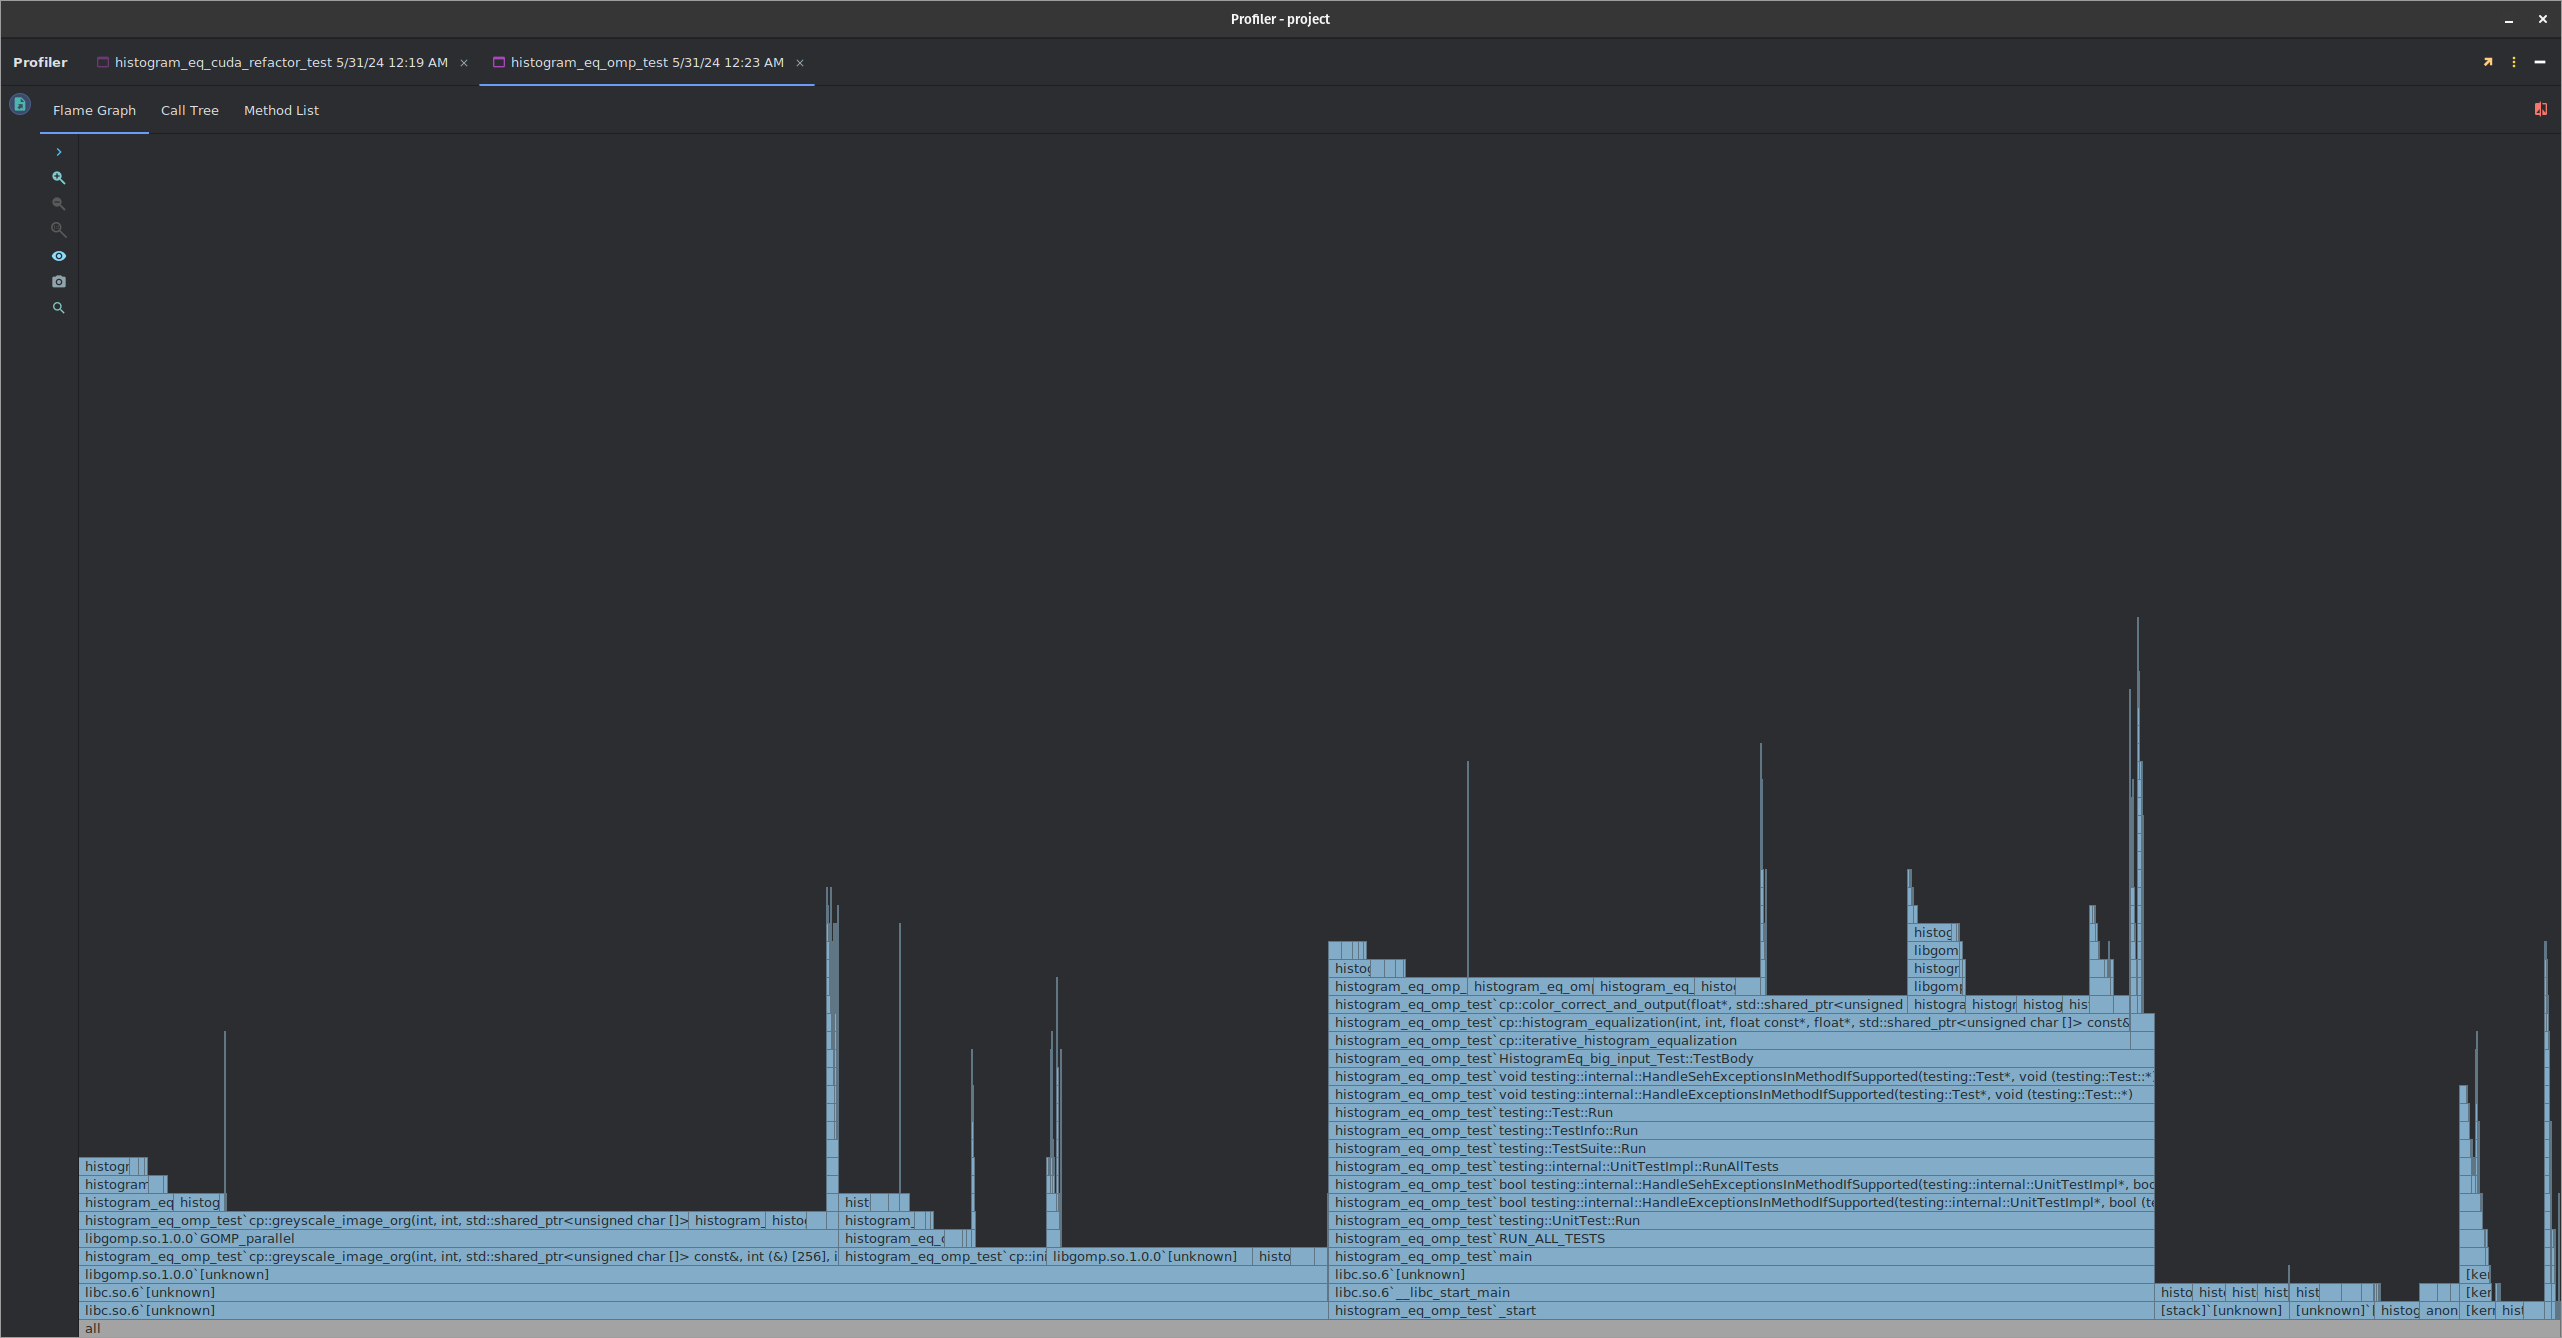
\includegraphics[width=0.8\linewidth]{vizs/omp_profiler.png}
    \captionof{figure}{CLion Profiler for the OpenMP version of the code.}
    \label{omp_profiler}
\end{center}

\subsection{CUDA}

Our last iteration of the histogram equalization function leveraged the CUDA library.

In our code, we didn't test the impact that the number of threads per block has on our performance, but it would have been an interesting phenomenon to observe. Our best estimates are that as the number of threads per block increases, performance would improve due to better utilization of GPU resources, until it reaches a threshold. Beyond this threshold, performance might degrade because of lack of proper GPU utilization or memory bottlenecks.

In that case, with threads per block set at 256 as previously mentioned, we can observe in Fig. \ref{just_cuda} that there is still an increase in the time it takes to process larger image sizes. 


\begin{center}
    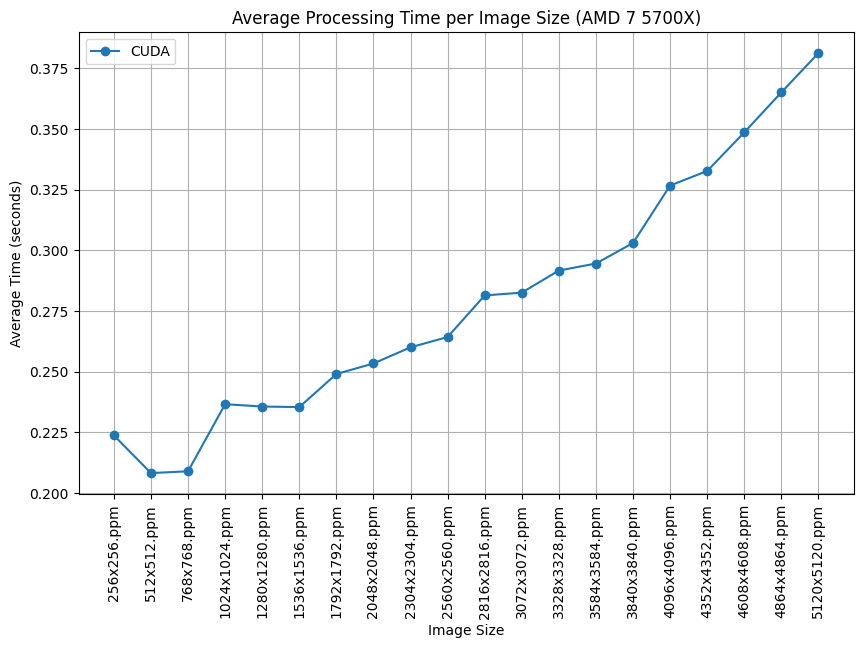
\includegraphics[width=0.8\linewidth]{vizs/just_cuda.png}
    \captionof{figure}{Average time spent in 4 iterations for various image sizes. CUDA Only. RTX 4070 Super.}
    \label{just_cuda}
\end{center}

This chart by itself doesn't convey much, except that unlike the previous two implementations, CUDA's processing time doesn't increase linearly with image size. This divergence from the linear trend suggests that in CUDA, the processing time may scale differently with the image size due to the parallel execution model and GPU architecture. It's possible that for certain image sizes, the GPU isn't fully utilized, leading to unexpected variations in processing time.

And if we take a look at the profiler output for the CUDA version, in Fig. \ref{cuda_profiler}, we don't see any specific bottlenecks that aren't already handled by CUDA itself.


\begin{center}
    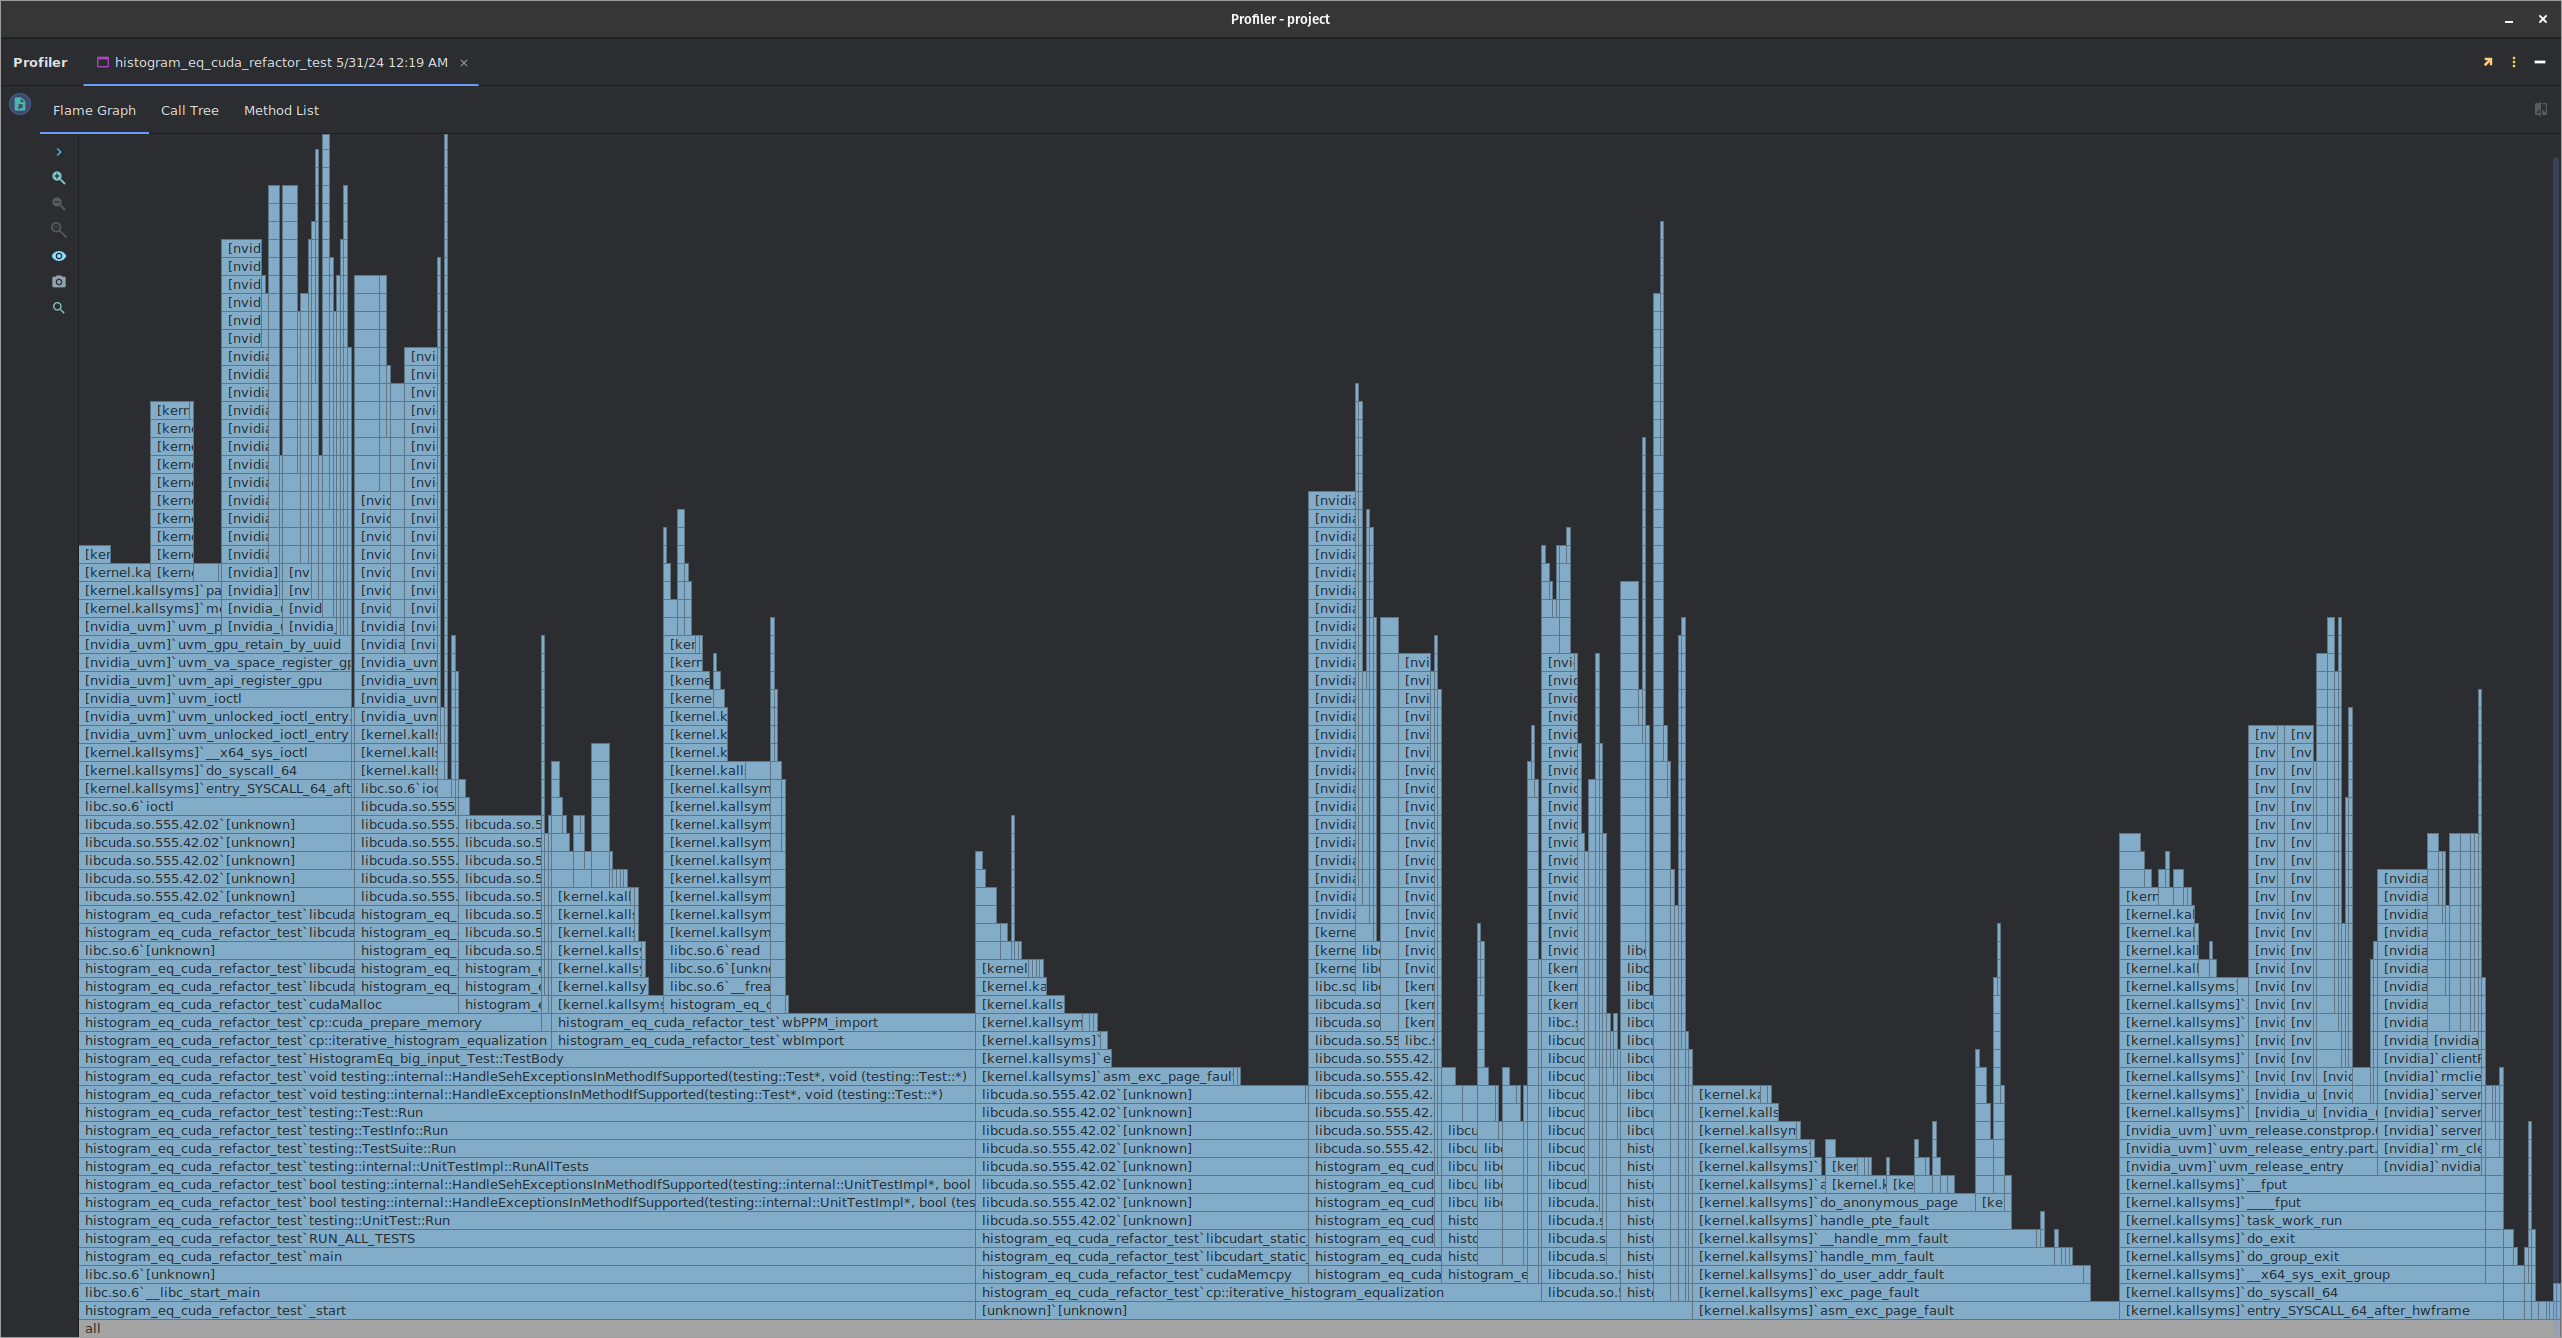
\includegraphics[width=0.8\linewidth]{vizs/cuda_profiler.png}
    \captionof{figure}{CLion Profiler for the CUDA version of the code.}
    \label{cuda_profiler}
\end{center}

When comparing CUDA to the other two implementations, we notice two distinct situations in Fig. \ref{processing_time_amd}:

\begin{center}
    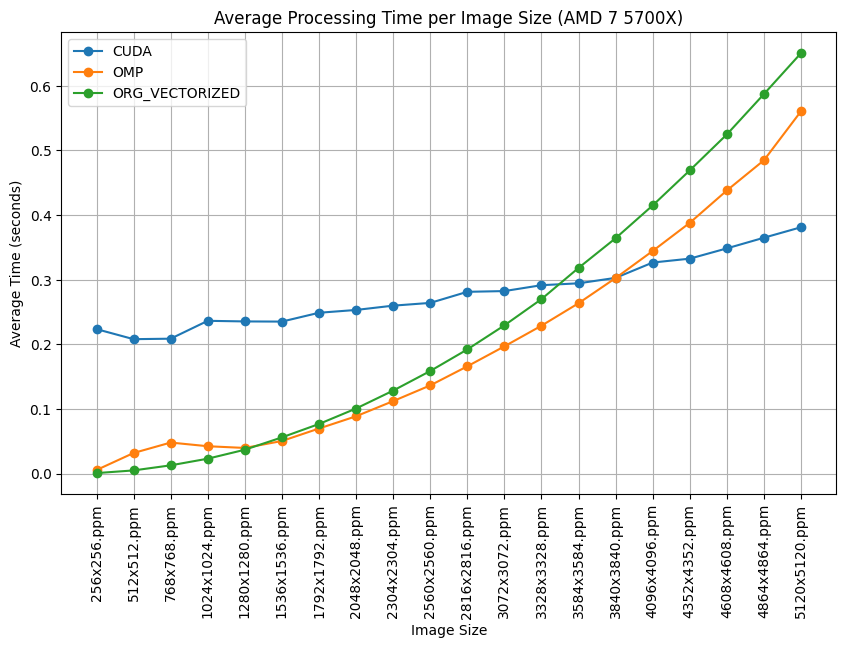
\includegraphics[width=0.8\linewidth]{vizs/amd_output.png}
    \captionof{figure}{Average time spent in 4 iterations for various image sizes. AMD 7 5700X + RTX 4070 Super.}
    \label{processing_time_amd}
\end{center}

Initially, there's a phase where the overhead of transferring data to and from the GPU, and processing it, is greater than executing the same code on the CPU using multi-processing techniques. However, there comes a point where the computational load of iterating over millions of pixels on the CPU becomes too heavy for it to handle. As shown, while both the sequential and OpenMP versions exhibit a curved growth pattern, CUDA progresses steadily. Unfortunately, beyond a certain point, running four iterations on images larger than our maximum size becomes too time-consuming. However, we can confidently say that while OpenMP and the sequential version struggle to handle these larger images, CUDA will likely continue to manage them effectively, provided there is enough memory available in the system.

\section{Conclusions}

\section{Acknowledgments}
I ( Tomás Mondim ) would like to thank student James Hertz, because in the final phase of the project, I was unable to go to the university to meet with the professor to solve some problems I encountered while running the project on the server. James dedicated several hours of his time to help me resolve these issues.

\section{Individual Contributions}
\begin{itemize}
    \item Tomás Mondim (0\%) and Cláudio Guerra (100\%): OpenMP Implementation
    \item Tomás Mondim (40\%) and Cláudio Guerra (60\%): CUDA Implementation
    \item Tomás Mondim (50\%) and Cláudio Guerra (50\%): Report Implementation
\end{itemize}

\section{Comments, Critics, and Suggestions}

Setting up CUDA in CMakeLists shouldn't be this hard. - Cláudio Guerra.

\end{document}